\chapter{Elements}
\label{sec:elements}

% \begin{importantbox}
% Add a better intro to the elements chapter.
% \end{importantbox}

This review does not attempt to catalogue every advance in robotic machine learning or its neighboring disciplines.  Instead, it focuses on the core theoretical foundations and key paradigms that enable \ac{VLA} models, \ac{RL}, and classical robot control to interoperate.

\section{Classical Control Theory}
\epigraph{``Every aspect of learning or any other feature of intelligence can in principle be so precisely described that a machine can be made to simulate it.''}{John McCarthy, \textit{Proposal for the Dartmouth Conference} (1955)}

Classical control theory provides the mathematical foundations for regulating dynamical systems. Early work formalized the feedback control paradigm, exemplified by James Clerk Maxwell’s analysis of governors in 1868 (ensuring stability of steam engine speed regulators). The field coalesced mid-20th century with rigorous stability criteria (e.g. Lyapunov functions) and optimal control formulations. A landmark contribution was dynamic programming that came from Bellman’s principle of optimality, which introduced recursive value functions for optimal decision-making over time \cite{BELLMAN1952}. \textcite{BELLMAN1952} showed that an optimal policy can be derived by backward induction on a value function, yielding what is now known as the Bellman equation. This paved the way for optimal control in continuous dynamics: Pontryagin’s Maximum Principle (1962) provided first-order optimality conditions for control trajectories, and \textcite{KALMAN1960} introduced the Linear Quadratic Regulator, giving closed-form optimal feedback for linear systems via solutions of the Riccati equation. Together, these developments established that controllability and observability (concepts first articulated by Kalman) are crucial system properties for design. Classical control also produced robust, easy-to-implement strategies like the PID controller with tuning rules from \textcite{ZIGOPTCONTROL1942}, which, though heuristic, became ubiquitous in engineering. In summary, classical control theory contributed a rich set of analytical tools (stability criteria, frequency-domain analysis, optimal control theory) that form the backbone for modern robotic control systems. These methods assume known system models; challenges in modeling and high-dimensionality later motivated data-driven and learning-based approaches.

% \begin{importantbox}[blue]{PCA}
% we'll talk about principal component analysis here, and make sure that it ties in nicely to classical control theory.  the link might be something to do with Manifold 
% \end{importantbox}

\section{Deep Learning}
% \epigraph{``Meaning lies as much in the structure of things as in their content.''}{Douglas R. Hofstadter, \textit{Gödel, Escher, Bach} (1979)}

\begin{flushright}{\slshape    
    \textit{Meaning lies as much in the \\
    structure of things as in their content.}} \\ \medskip
    --- \textsc{Douglas R. Hofstadter} \cite{GEB1999}
\end{flushright}

\bigskip

Alan Turing's 1950 essay posed the question ``Can machines think?'' and introduced the imitation game, later called the Turing Test, as an operational criterion for intelligence \cite{TURING1950}. Early AI research embraced symbolic reasoning, producing search-based solvers, the Physical Symbol System Hypothesis \cite{NEWELL1976} and rule-driven expert systems. Limitations in perception and scaling spurred the statistical turn: perceptrons \cite{PERCEPTRON1958}, the universal approximation theorem \cite{SIGMOID1989}, back-propagation \cite{BACKPROP1986} and probabilistic graphical models \cite{PEARLPROB1988}. The deep learning era began when GPUs enabled AlexNet to win ImageNet 2012 \cite{IMAGENET2012}, quickly followed by residual networks \cite{RESNET2016} and sequence models such as LSTM \cite{LSTM1997}. In reinforcement learning, Deep Q-Networks achieved human-level Atari play \cite{MNIH2015}. The transformer architecture \cite{ATTENTION2023} catalyzed large language models such as GPT-3 \cite{GPT32020} and GPT-4, while multimodal pretraining produced models such as CLIP \cite{CLIP2021}. Today’s state-of-the-art systems combine self-supervised pretraining, scaling laws and prompt-based adaptation, pushing AI toward generalist, vision-language-action agents.

\subsection{Representation Learning}

Deep learning must discover useful representations from data. For example, Figure \ref{fig:representations} shows that classes are not separable in Cartesian coordinates $(x,y)$ but become linearly separable in polar coordinates $(r,\theta)$. While the mapping  $f\colon(x,y)\mapsto(r,\theta)$ follows directly from coordinate geometry, a deep learning model must infer its own optimal transformation $f$ without relying on any predefined axioms.

\begin{figure}[ht]
    \centering
    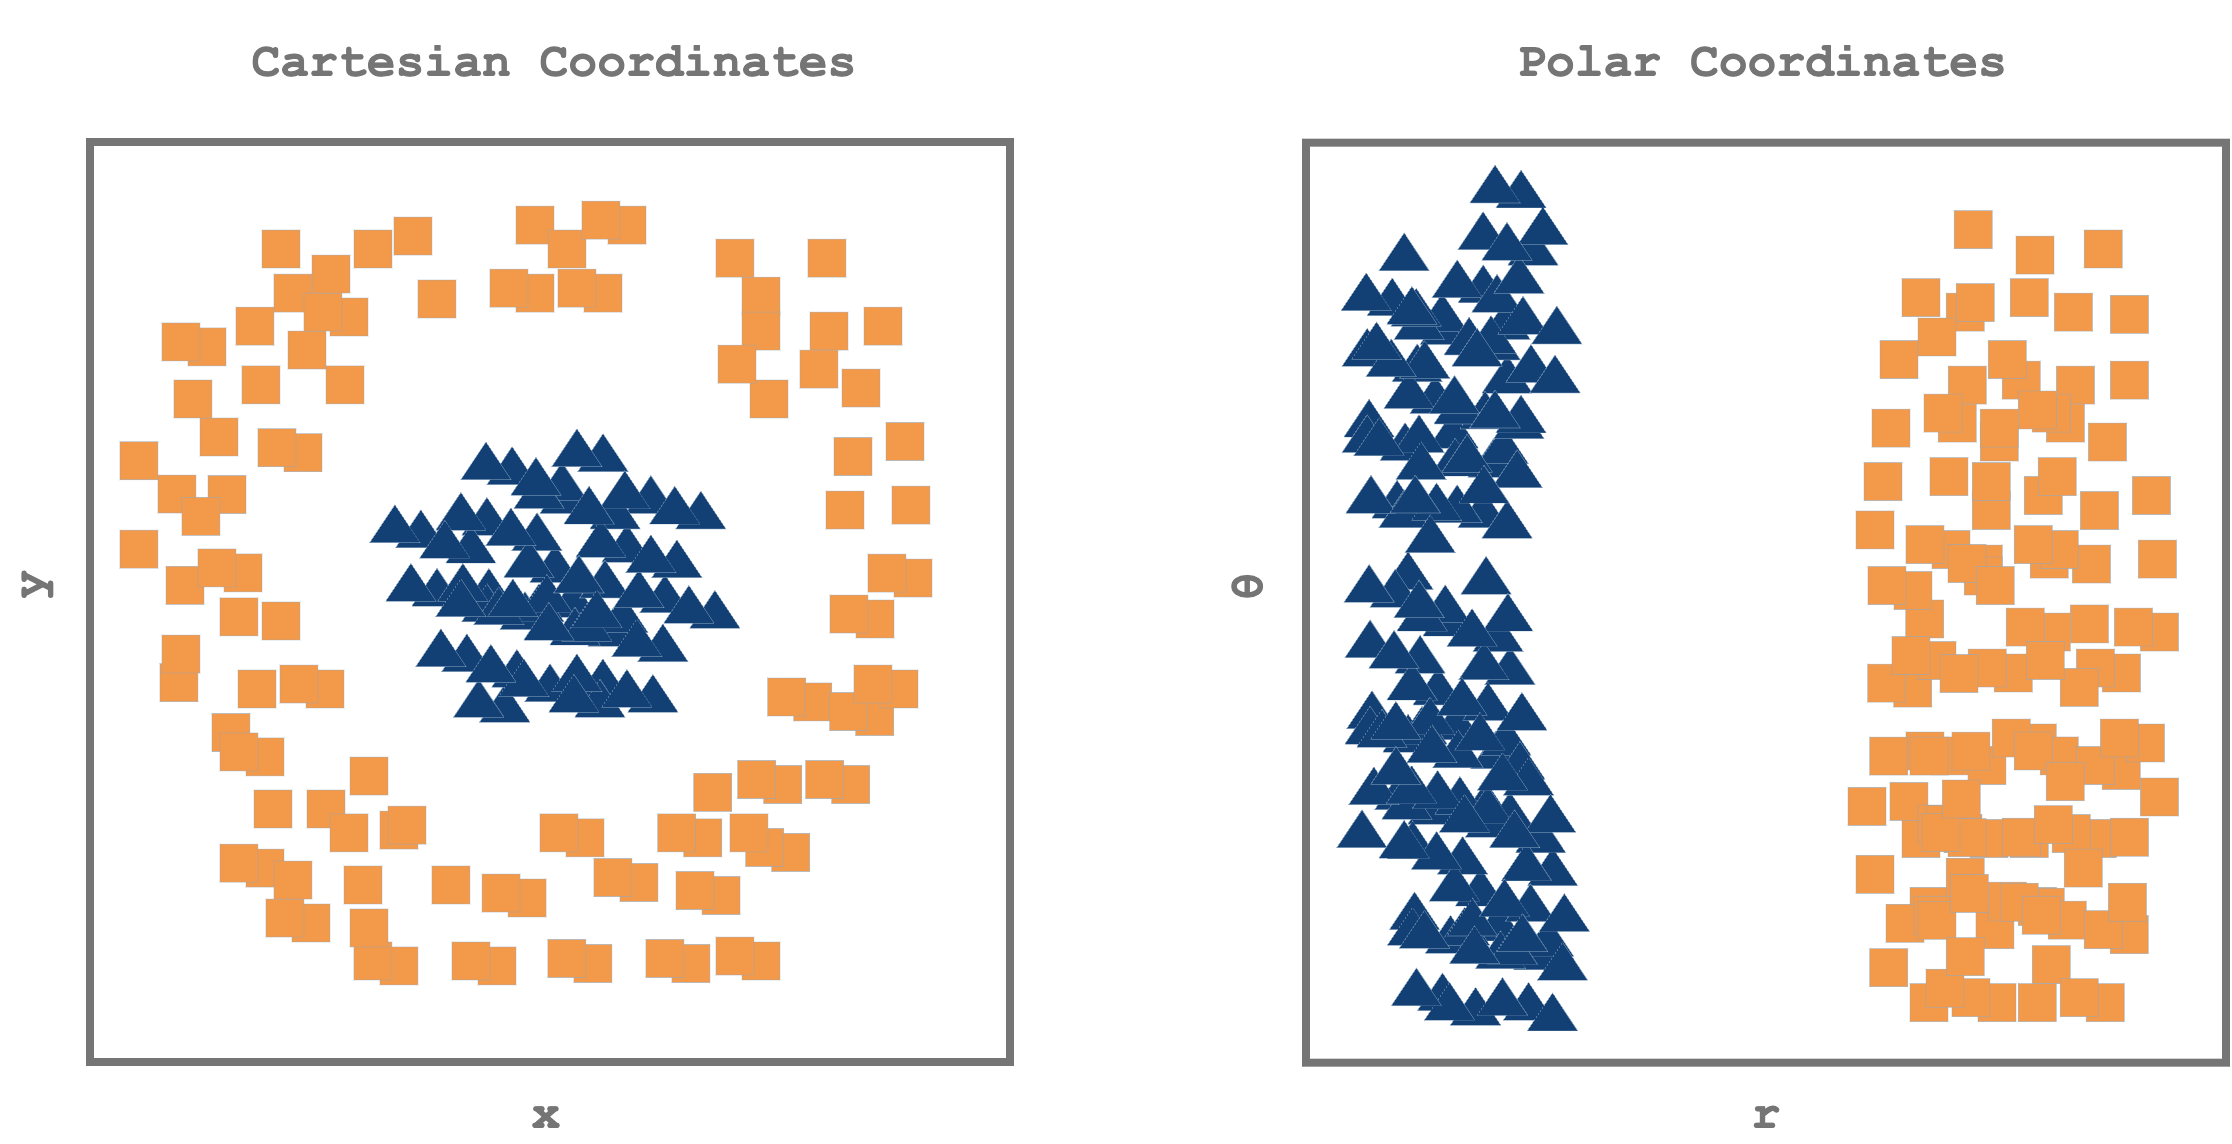
\includegraphics[width=0.8\textwidth]{Figures/representations.png}
    \caption{Illustration of representation learning: in Cartesian space the blue inner cluster and orange outer ring require a complex boundary, but in polar coordinates they separate linearly along the radial axis.}
    \label{fig:representations}
\end{figure}

The world's complexity could not be modeled linearly, often requiring non-linearity to capture complex relationships between concepts. For instance, separating foreground objects from camouflage backgrounds often requires a non‑linear transformation such as a colour‐opponent space (e.g.\ CIELAB \cite{CIELAB2018}), which renders the decision boundary almost linear.

A common task of a supervised learning\footnote{Self‑supervised and contrastive objectives have become the default pre‑training paradigm for large‑scale models, but supervised
examples remain essential for calibration and evaluation.} system is to predict an output $\hat{\bold{y}} \in \mathbb R^k$ from some input $\bold x \in \mathbb R^d$. That process can be called $f$ where $\hat{\bold{y}} = f(x)$. With the following simple equation,
\begin{equation}
    \hat{\bold{y}} = \sigma(W\bold x + \bold b),
    \label{eq:neuron}
\end{equation}
we can tweak the values of $W, b$ and $\sigma$ to produce accurate estimates of $\hat{y}$ if we have a valid training set to work with $\mathcal{D} = \{\bold x^{(i)}, \bold y^{(i)}\}^N_{i=1}$ where $\bold x^{(i)} \in \mathbb R^d$ and $\bold y^{(i)} \in \mathbb R^k$. $W$ is weight, $\bold b$ is bias and $\sigma$ is a non-linear activation function such as ReLU or sigmoid.

Stacking multiple units of \cref{eq:neuron} together into $L$ layers provides the depth necessary for more complicated representations to emerge.
\begin{equation}
    \bold a^{(\ell)} = \sigma(W^{(\ell)}\bold a^{(\ell -1)} + \bold b^{(\ell)}),\quad \ell = 1,\ldots ,L.
    \label{eq:layer}
\end{equation}

The final prediction can be computed by running a forward-pass from $\bold a^{(0)} = \bold x$ all the way through $L$ layers to $\hat{\bold y} = \bold a^{(L)}$. The first prediction will not be very good since the set of weights $W^{(\ell)} \in \mathbb R^{n_{\ell}\times n_{\ell - 1}}$ have not been updated to bring the predictions as close as possible to the original training set $\mathcal D$. This can be solved by minimizing the loss between $y_i$ and $\hat{y}_i$ with a loss function 
\begin{equation*}
    J(\theta) = \dfrac{1}{N} \sum_{i = 1}^{N} L(\bold{y}^{(i)},  \hat{\bold{y}}^{(i)}).
\end{equation*}
Typically this is performed by a gradient-based optimization, namely gradient-descent where there parameters are updated via $\theta \leftarrow \theta -\eta \nabla_{\theta}J(\theta)$ where $\theta \in \{W^{(\ell)}, b^{(\ell)}\}^L_{\ell=1}$ and $\eta$ configures the \textit{learning rate}.

Running this algorithm separately to improve the predictive $f$ capability is the machine learning; which becomes deep learning when $L > 2$.

The deeper the network the more complicated features it can learn. However the deeper it becomes the more parameters there are to train and the harder it is to \textit{understand} what is actually going on inside the black box $f$. 

Residual connections~\cite{RESNET2016} enable gradients to bypass
poorly conditioned layers, effectively learning a series of
incremental $\Delta f$ refinements rather than an entire mapping from
scratch.  Formally, a residual block learns
$\mathbf{y} = f(\mathbf{x}) + \mathbf{x}$, where
$f$ is a small stack of convolutions and
$\mathbf{x}$ is the identity shortcut.  This simple reformulation
mitigates vanishing gradients and allows networks hundreds of layers
deep to converge reliably.

\subsection{Convolutional Neural Networks} 

Building on \cref{eq:layer}, neural networks can learn to predict outputs from a primitive vector-based dataset $\mathcal D$, but a useful extension is to give a capable network the ability to see in the real world. 

Take an input (also called feature map) $X \in \mathbb R^{H\times W \times C}$ with $W, H$ and $C$ as the width, height and channel depth\footnote{An \ac{RGB} image has $C = 3$ for red, green and blue.} of the image. Passing even a small \ac{RGB} map $X\in \mathbb R^{100\times 100\times 3}$ through a fully connected layer would require 10,000 weights per neuron. This quickly becomes intractable for large enough feature maps so they must be compressed with minimal feature loss; a prime function of a \ac{CNN}.

The feature map is convolved with a kernel $K \in \mathbb R^{k_H\times k_W \times C \times C'}$, producing the $(i,j)$th compressed output as (where $i$ and $j$ correspond to individual pixels),
\begin{equation*}
    Y_{i,j,c}^{(\ell)} = (X * K)_{i,j,c} = 
\sum_{u=1}^{k_H}\sum_{v=1}^{k_W}\sum_{c=1}^{C}
X_{i+u-1,\,j+v-1,\,c}^{(\ell - 1)}\;K_{u,v,c',c}^{(\ell)}.
\end{equation*}

The final output of each layer with kernel  $K^{(\ell)}$ and bias $b^{(\ell)}$is,
\begin{equation*}
    A_{i,j,c}^{(\ell)} = \sigma\left(Y_{i,j,c}^{(\ell)} + b^{(\ell)}\right),
\end{equation*}
where $\sigma$ is a non-linearity. Stacking $A^{(\ell)}$  gives the next layer’s input of shape $(H^{(\ell+1)}, W^{(\ell+1)} , C^{(\ell+1)})$ which are depend on the padding $P$ and stride $S$ parameters,
\begin{equation*}
    H^{(\ell)} = \dfrac{H^{(\ell - 1)} - k_H +2P}{S} + 1, \quad
W^{(\ell)} = \dfrac{W^{(\ell - 1)} - k_w +2P}{S} + 1.
\end{equation*}

\paragraph{Pooling.} 

To reduce spatial size the input $X \in \mathbb R^{H\times W \times C_{\text{in}}}$ to something smaller, pixel regions are \textit{pooled} into smaller subregions and passed to the next layer (red layers in \cref{fig:conv_arch}). This is often taken over the max or average of a $p\times p$ patch,
\begin{equation*}
P_{i,j}^{(\ell)} = \max_{0\le u,v < p} A^{(\ell)}_{ip+u, jp+v},\quad \text{or}\quad P_{i,j}^{(\ell)} = \dfrac{1}{p^2}\sum_{0\le u,v < p} A^{(\ell)}_{ip+u, jp+v}.
\end{equation*}

\begin{figure}[ht]
    \centering
    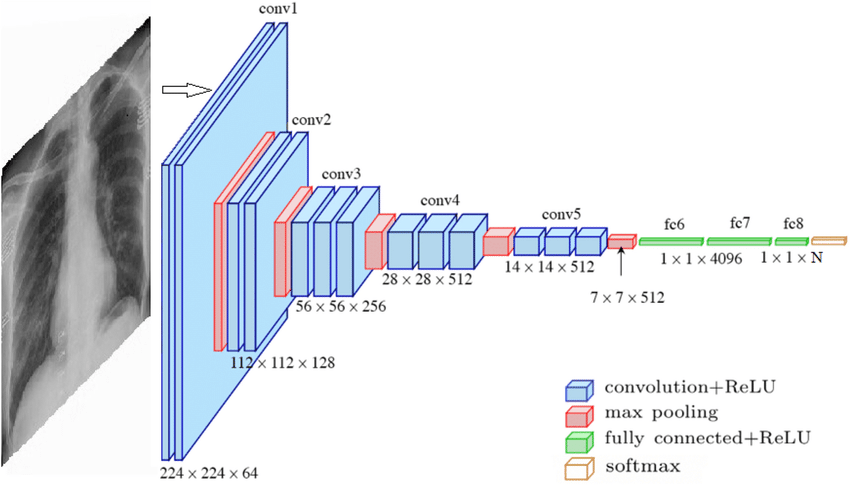
\includegraphics[width=0.7\textwidth]{Figures/conv-arch.png}
        \caption{Architecture of a deep convolutional network showing five convolutional blocks (blue: conv+ReLU, red: max-pooling) that transform a 224 × 224 × 3 input into a 7 × 7 × 512 feature map, followed by three fully connected layers (green: ReLU, orange: softmax) producing an $N$-way classification. Adapted from \textcite{CONVNETARCH2021}.}
    \label{fig:conv_arch}
\end{figure}

\paragraph{Fully Connected Layers.}

Convolutions and pooling are performed until the feature map has been reduced enough to a fully connected layer learn the features.

The final feature map is flattened into a vector $\bold h \in \mathbb R^D$ where $D$  is the product of the dimensions of the last pooling layer (green layers in \cref{fig:conv_arch}). Then final output is calculated using the softmax $\hat{\bold{y}} = \text{softmax}(W_{fc}\bold h+\bold b_{fc})$ which can be trained using  $\theta \leftarrow \theta - \eta \nabla_{\theta}L(\theta)$.

The \ac{CNN} was conceived by \textcite{CONV1980}, however it was \textcite{CONV1989} that introduced end-to-end supervised learning with trainable convolutional filters via backpropagation, formalized weight sharing, and demonstrated state-of-the-art handwritten digit recognition.

\paragraph{Vanishing Gradients.}

As networks grow deeper, gradients propagated through many layers tend to shrink toward zero, hindering effective weight updates in early layers. ResNets overcome this by adding identity skip connections,
\begin{equation*}
    A^{(\ell + 1)} = f(A^{(\ell)}) + A^{(\ell)},
\end{equation*}
that let gradients flow unimpeded through shortcut paths. This simple modification enables training of ultra-deep \ac{CNN} models without loss of signal \cite{RESNET2016}.

\paragraph{Compound Scaling.}

Scaling up \acp{CNN} to more layers can result in better accuracy as seen from ResNet-18 to ResNet-200 \cite{RESNET2016}. Although poorly understood, \ac{CNN} scaling can occur across three dimensions: width \cite{WIDERESNETS2016}, depth \cite{RESNET2016} or resolution scaling \cite{GPIPE2019}. \textcite{EFFICIENTNET2020} formulated a unified scaling framework by using single compound coefficient $\phi$ to scale depth, width and resolution from their baseline values $d^{(0)} = L, w^{(0)} = W$ and $r^{(0)}$. Each increment of $\phi$ roughly doubles compute by enforcing $ \alpha\,\beta^{2}\,\gamma^{2}\approx 2$, where $\alpha,\beta,\gamma>1$ are constants. The resulting dimensions are \begin{equation*}
(d,w,r) = \bigl(d^{(0)},\,w^{(0)},\,r^{(0)}\bigr) \odot \bigl(\alpha^{\phi},\,\beta^{\phi},\,\gamma^{\phi}\bigr).
\end{equation*}

\subsection{Autoencoders}

\acp{AE} are representation learning architectures that works in two parts: an encoder function $\bold h = f(\bold x)$ and decoder that produces reconstruction $\bold r = g(\bold h)$ with parameters $\{\theta_f, \theta_g\}$. It consists of a hidden layer $\bold h$ that describes the latent representation of the input to learn $g(f(\bold x)) \approx \bold x$ by, minimizing a loss 
\begin{equation*}
\min_{\theta_f, \theta_g} L(\bold x, g(f(\bold x)).
\end{equation*}

\acp{AE} come in many different forms, such as Sparse \acp{AE} $\min_{\theta_f, \theta_g} L(\bold x, g(f(\bold x)) + \Omega(\bold h)$ with a sparsity penalty $\Omega(\bold h)$ for classification \cite{SAE2024}, Denoising \acp{AE} $\min_{\theta_f, \theta_g} L(\bold x, g(f(\bold{\tilde{x}}))$ with $\bold{\tilde{x}}$ being a corrupted copy of $\bold x$ for filtering noise \cite{DAE2015} and others. \acp{VAE} are of particular interest where instead of propagating signals through a latent bottleneck $\bold h$ they impose a probabilistic prior on the latent space, 
\begin{equation*}
\min_{\theta_f,\theta_g}
\mathbb{E}_{f(\bold h\mid\bold x)}
[L(\bold x,\, g(\bold h))]
+ D_{\mathrm{KL}}\!\bigl(
  f(\bold h\mid\bold x)\,\|\,\mathcal{N}(0, I)
\bigr)
\end{equation*}
from $f(\bold h \mid\bold x) \sim \mathcal{N}(\mu, \sigma^2I)$, which yields continuous, disentangled representations that can be smoothly sampled to generate novel data like images \cite{VAE2020}\footnote{The \ac{KL} divergence measures how a distribution $q(\mathbf z)$ departs from a reference $p(\mathbf z)$: $D_{\mathrm{KL}}(q\,\|\,p)=\int q(\mathbf z)\log\bigl(\frac{q(\mathbf z)}{p(\mathbf z)}\bigr)\,d\mathbf z$. It is always non-negative, equals $0$ only when $q=p$, and is asymmetric \cite{KLDIV1951}.}.

\section{Transformers}

Sequence transduction modelling has been important for the fields of language translation and next token prediction,
\begin{align*}
    (x_1, x_2, \ldots, x_T) &\mapsto (\hat{y}_1, \hat{y}_2, \ldots, \hat{y}_{T'}) \\
    (x_1, x_2, \ldots, x_T) &\mapsto (\hat{y}_{T+1}),
\end{align*}
where $x_t \in \mathcal V_x, y_t \in \mathcal V_y$. \textcite{LSTM1997} introduced the \ac{LSTM} architecture for \acp{RNN}. \textcite{SEQ2SEQ2014} later used LSTMs for sequence-to-sequence learning. Calculating each hidden state $h_t = f(x_t, h_{t-1})$ requires the preceding state, which limits parallelism across time steps.

With the introduction of the transformer by \textcite{ATTENTION2023} paralleization was now possible with a new model architecture that calculated the self-attention between all tokens $(x_1, x_2, \ldots, x_T)$ in a sequence. Self-attention is computed by compiling three vectors: $\bold k = [k_1, k_2, \ldots, k_T]^T$ encoding the position of each token, $\bold q = [q_1, q_2, \ldots, q_T]^T$ the starting token, and $\bold v = [v_1, v_2, \ldots, v_T]^T$ a set of value vectors that store the information content of each token\footnote{In the literature $\bold k, \bold q$ and $\bold v$ are normally expressed as matrices $K, Q$ and $V$. Vectors were used here for exposition to highlight the per-token computation; in practice these are batched as matrices to enable efficient parallel processing.}. Mathematically, attention is the weighted sum\footnote{The sum of the product $\bold q_k \cdot \bold k_t$ should be evenly diffused to avoid softmax generating one-hot vectors, where very large values in the softmax can drown out the smaller values. We don’t want that. Hence it’s safer to scale the dot product i.e., $\bold q_k \cdot \bold k_t / \sqrt{d_k}$ where $d_k$ is the attention head size \cite{ATTENTION2023}.} from query vector $\bold q_k$,
\begin{equation*}
    \bold z _k = \text{Attention}(\bold q_k, \bold k, \bold v) = \sum^T_{t=0} \text{softmax}(\bold q_k \bold k_t^T) \bold v_t.
\end{equation*}

With the benefits of high parallezibility come from stacking multiple attention heads together into a multihead attention block,
\begin{align*}
    \text{MultiHeadAttention}(\bold q_k, \bold k, \bold v) &= \text{concat}(\text{head}_1(\bold q_k), \ldots,\text{head}_h(\bold q_k)) \\
    \text{where } \text{head}_i(\bold q_k) &= \text{Attention}(W_i^{Q} \bold q_k, W_i^{K} \bold k, W_i^{V} \bold v)W^O.
\end{align*}
Here the parameter matrices are $W_i^Q \in \mathbb{R}^{d_{\mathrm{model}}\times d_k}, W_i^K \in \mathbb{R}^{d_{\mathrm{model}}\times d_k}, W_i^V \in \mathbb{R}^{d_{\mathrm{model}}\times d_v}$ and $W^O \in \mathbb{R}^{h\,d_v\times d_{\mathrm{model}}}$.

This ability to capture long-range phenomena became noteworthy as language transduction models began to sound more human-like.

\begin{figure}[ht]
    \centering
    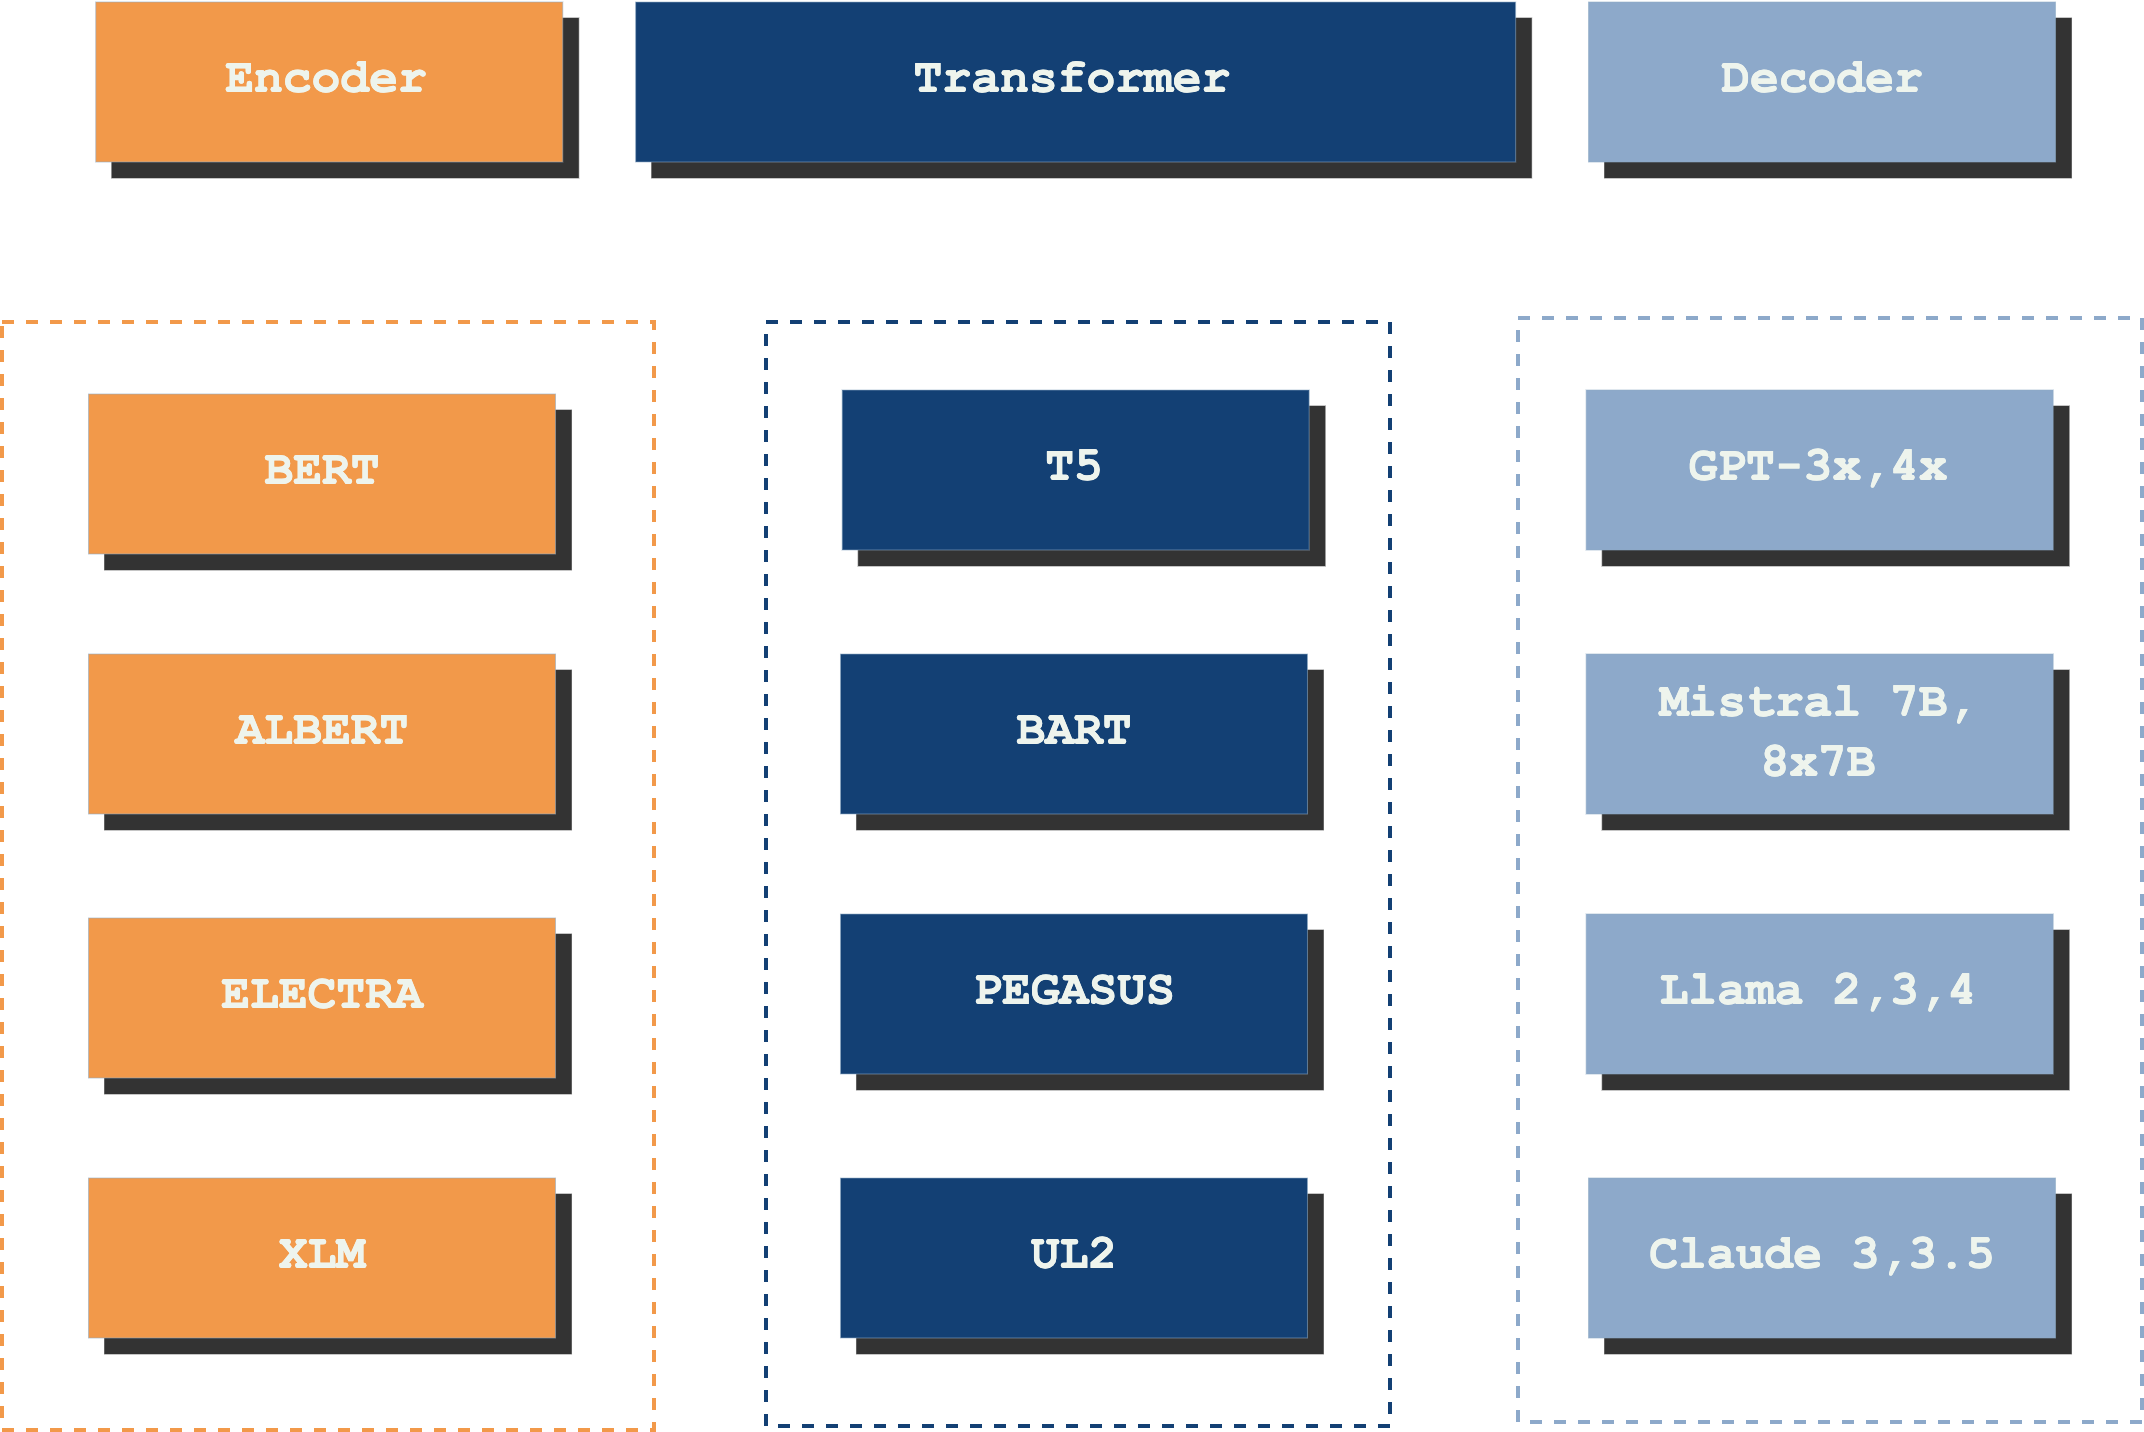
\includegraphics[width=0.8\textwidth]{Figures/transformers.png}
    \caption{Overview of transformer model families grouped by architecture. \textit{Left}: encoder only (BERT, ALBERT, ELECTRA, XLM). \textit{Middle}: encoder-decoder (T5, BART, PEGASUS, UL2). \textit{Right}: decoder only (GPT-3x/4x, Mistral 7B/8×7B, Llama 2/3/4, Claude 3/3.5).}
    \label{fig:transformers}
\end{figure}

\subsection{Large Language Models} 
\label{sec:llms}

Different types of transformers have emerged most notable decoder-only \cite{GPT32020}, encoder-only \cite{BERTGPT2023} and a encoder-decoder mix \cite{BART2019} as shown in \cref{fig:transformers}. Each has its advantages and disadvantages. Decoder-only transformers tend to perform better at open‑ended sequence generation, code synthesis and in‑context few‑shot prompting due to their autoregressive training. Encoder-only transformers perform better at discriminative tasks because of their \ac{MLM} bidirectional training.

Transformers, like any other neural network, can only take real numbers as inputs. Therefore translating language to numerical format, also known as tokenizing, can meaningfully dictate the capabilities of the language model. Nuemrous tokenizing schemes are employed today most notably WordPiece used by \ac{BERT} \cite{WORDPIECE2021} and \ac{BPE} used by \ac{GPT}-series \cite{BPE2024}. Formally, a tokenizer is a mapping $T:\Sigma^*\to V^*$ from an input string over alphabet $\Sigma$ to a sequence of tokens in vocabulary $V$ (with $|V|$ fixed). For any word $w\in\Sigma^*$ we write  
$T(w)=(s_1,s_2,\dots,s_k)$, where $s_i\in V$ and $w=s_1\circ s_2\circ\cdots\circ s_k$. Each token $s_i$ is then mapped to an integer ID via a lookup $f:V\to\{1,\dots,|V|\}$.

\paragraph{Byte-Pair Encoding.} Start with $V_0=\Sigma$ and counts $c_0(a,b)$ for every adjacent symbol pair $(a,b)$. At each merge step $t=1,\dots,N$, pick $(a^*,b^*)=\arg\max_{(a,b)}c_{t-1}(a,b)$,  
then define a new symbol $x=a^*b^*$ and update $V_t=V_{t-1}\cup\{x\}$ and counts by replacing all occurrences of $(a^*,b^*)$ with $x$. After $N=|V|-|\Sigma|$ merges, $V_N$ has the desired size. Tokenization greedily matches the longest symbol in $V_N$ at each step.

\paragraph{WordPiece.} Given corpus $C$, learn $V$ by maximizing the data likelihood under a subword model. One often maximizes  
\begin{equation*}
\max_V\prod_{w\in C}\sum_{(s_1,\dots,s_k)=w}\prod_{i=1}^k p(s_i\mid s_{<i}),
\end{equation*}
where $p(s_i\mid s_{<i})$ is estimated from subword counts. In practice a greedy heuristic adds the subword that most increases the log-likelihood until $|V|$ is reached.

% TODO
% \begin{importantbox}
% Backfil
% \end{importantbox}

\subsection{Vision Transformers} 

While the Transformer architecture \cite{ATTENTION2023} has become the de-facto standard for natural language tasks, it has proven to be effective at computer vision tasks when paired with an effect tokenizer and a high data regime (14M-300M images) \cite{16x162021}. Propagating an image $\bold x \in \mathbb R^{H\times W\times C}$ through a \ac{ViT}, requires it to be flattened into a linear sequence of patches $\bold x_p \in \mathbb R^{N\times (P^2C)}$ where $(P,P)$ is the resolution of each image patch and $N = HW/P^2$ is the resulting number of patchs. Patches can then be treated equal to word tokens in a natural language context allowing the model to be trained on tasks like image classification in a supervised fashion. \acp{ViT} have shown remarkable generalization when trained on a large corpus of images, even outperforming \acp{CNN} \cite{16x162021}.

\subsection{Vision Language Models} 
\label{sec:vlms}

\acp{VLM} extend the Transformer architecture to jointly model images and text. Modern \acp{VLM} fall into four broad families based on their pretraining objectives. Pioneering efforts such as Visual-\ac{BERT} and ViL\ac{BERT} embed image regions and words into a shared Transformer. They are trained on (a) masked token modelling to predict missing words or image regions, and (b) image–sentence matching to decide whether a caption describes an image \cite{VISUALBERT2019,VLBERT2019}.

\paragraph{Contrastive–based VLM.}
Models like \ac{CLIP} train separate image and text encoders on hundreds of millions of image–caption pairs using an InfoNCE loss. Matched pairs are pulled together in a shared embedding space while mismatched pairs are pushed apart. At inference, text prompts can retrieve semantically aligned images in zero-shot fashion (e.g.\ \ac{CLIP} with ResNet-101 attains 76.2\% zero-shot ImageNet accuracy) \cite{CLIP2021}.

SigLIP replaces \ac{CLIP}'s softmax-normalized contrastive loss with a pairwise sigmoid loss 
\begin{equation*}
    L_{\mathrm{sig}} = -\dfrac{1}{|\mathcal B|}\sum_{(i,j)\in\mathcal B}\bigl[y_{ij}\log\sigma(z_i\!\cdot\!z_j)+(1-y_{ij})\log(1-\sigma(z_i\!\cdot\!z_j))\bigr],
\end{equation*}
operating per image–text pair without global normalization and yielding improved zero-shot accuracy and batch-size scalability \cite{SIGLIP2023}.

\paragraph{Masking–based VLM.}
Masking approaches view \ac{VLM} pretraining as cross-modal denoising. FLAVA employs three Transformer encoders (image, text, multimodal) and combines unimodal/multimodal masked modelling with a contrastive loss, achieving state-of-the-art results on over 35 vision, language, and multimodal benchmarks after pretraining on 70 M image–text pairs \cite{FLAVA2022}. MaskVLM extends this by masking raw pixels and text tokens simultaneously, using each modality to help reconstruct the other \cite{MASKEDVLM2023}.

\paragraph{Generative–based VLM.}
Generative \acp{VLM} learn to produce text and/or images directly. CoCa adds a caption-generation loss atop contrastive training, enabling tasks like \ac{VQA} without extra fusion modules; it is pretrained on over 1 B images with alt-text annotations \cite{COCA2022}. Mixed-modal autoregressive models such as CM3Leon interleave image and text tokens in a single decoder, supporting both image-to-text and text-to-image generation with retrieval-augmented pretraining and supervised fine-tuning \cite{CM3LEON2023}.

\paragraph{VLM from Pretrained Backbones.}
To reduce compute and data demands, many \acp{VLM} map frozen pretrained encoders into each other's space. Frozen maps visual features (NF-ResNet-50) into a frozen 7B-parameter \ac{LLM}, fine-tuning only a lightweight projection head on Conceptual Captions for rapid zero-/few-shot multimodal capabilities \cite{FROZENLANGUAGE2021}. Mini\ac{GPT}-4 aligns BLIP-2's Q-Former+\ac{ViT} image embeddings to a Vicuna \ac{LLM} via a small projector trained on $\sim$5 M image–text pairs and an instruction-tuning step \cite{MINIGPT42023}.

\section{Reinforcement Learning}
\label{sec:rl_theory}

\begin{flushright}{\slshape    
    \textit{The most important thing for AI \\
    is to have systems that can \\
    learn from experience, like humans do.}} \\ \medskip
    --- \textsc{Yann LeCun} \cite{LECUNINTERVIEW2018}
\end{flushright}

\bigskip

\ac{RL} is a reward-based paradigm in which an agent improves its behavior through trial and error. Unlike supervised learning, which relies on labeled input–output pairs to minimize a predefined loss, and unsupervised learning, which uncovers structure without external feedback, \ac{RL} uses scalar rewards to guide policy improvement over time.

\subsection{Formal Framework}

An \ac{RL} problem is modeled as a \ac{MDP} defined by a 5-tuple $(\mathcal{S}, \mathcal{A}, P, r, \gamma)$. The transition function is defined as $P: S\times A \rightarrow S$ and the reward function is $r: S\times A \rightarrow \mathbb R$. In general, for solving any agent-world \ac{RL} task:
\begin{enumerate}
    \item At each time $t$ the agents observe the current state $s_t \in \mathcal{S}$
    \item Selects the appropriate action $a_t \in \mathcal{A}$ to perform
    \item Environment returns a reward $r_t=  r(s_t, a_t)$
    \item Agent transitions to state $s_{t+1} = P(s_t, a_t)$
\end{enumerate}

The goal should be to follow (and create) a policy $\pi: S \rightarrow A$ that maximizes the accumulated reward over time $V^\pi(s_t)$. That policy $\pi(a|s)$ maps states to action probabilities with the return from time $t$ as
\begin{equation*} 
    G_t = \sum_{k=0}^\infty \gamma^k r_{t+k+1},
\end{equation*}
with $\gamma \in [0,1)$ as the discount factor applied to each successive reward $r_t$ determining whether the agent is myopic $(\gamma =0)$ and foresighted $(\gamma = 1)$.

The value $v$ of a state $s$ under a policy $\pi$ is expressed as $V_\pi(s_t)$ or $V^\pi(s_t)$ depending on the textbook,
\begin{equation*} 
    V^\pi(s) = \mathbb{E}_\pi\bigl[G_t \mid s_t = s\bigr],
\end{equation*}

and the action–value function is
\begin{equation*} 
    Q^\pi(s,a) = \mathbb{E}_\pi\bigl[G_t \mid s_t = s,\;a_t = a\bigr].
\end{equation*}

The optimal policy $\pi^*$ then satisfies
\begin{equation*} 
\pi^*(s) = \argmax_a Q^\pi(s,a).
\end{equation*}

The search for $a$ is the ultimate goal of any \ac{RL} agent. There are two predominant methods: (1) if we know $Q(s,a)$ then solve for $a = \argmax_a Q(s,a)$, referred to as value-based methods and (2) first find $\pi(s)$ to then sample $a \sim \pi(s)$, referred to as policy-based methods. These will be the focus of the remainder of \S\ref{sec:rl_theory}.

\subsection{Value-Based Methods}

\paragraph{TD Learning.}

\ac{TD} agents learn from experience over time (i.e., temporally). Modeling their impact on an environment as a function of the current state and action taken can provide enough stimulus to inform successive decisions, 
$$
V(s_t) \leftarrow V(s_t)+\underbrace{\alpha}_{\text{learning rate}}\underbrace{\left[\underbrace{r_{t+1}}_{\text{reward}} + \underbrace{\gamma V(s_{t+1})}_{\text{discounted value of next state}} - V(s_t)\right]}_{\text{temporal difference}}.
$$
An action $a_t$ that is taken in state $s_t$ at time step $t$ in accordance with policy $\pi$ is denoted as $Q_\pi(s_t,a_t)$ which is the action-value function. With the optimal policy $\pi^*$ one can arrive at the optimal action-value function,
$$
Q^*(s_t,a_t) = \max_\pi Q^\pi(s_t, a_t).
$$

\paragraph{Q-Learning.}

The agent maintains a table of action-value estimates, $Q(s,a)$, which it updates at each time step using the Bellman equation. This table records expected returns for every state–action pair and serves as a dynamic reference for decision making. Because updates are based on the highest-valued actions rather than the behavior policy $\pi$, this approach is classified as off-policy control \cite{QLEARNMULTIAGENT2015}.

\begin{algorithm}
\caption{Q‑Learning with Flexible Action‑Selection}
\label{alg:qlearning_flex}
\begin{algorithmic}[1]
  \Require learning rate $\alpha$, discount $\gamma$, episodes $M$
  \Require decay factors $\lambda$ (for $\varepsilon$) and $\kappa$ (for $\tau$)
  \Require \texttt{policyType} $\in\{\text{greedy},\ \varepsilon\text{-greedy},\ \text{softmax}\}$
  \State Initialise $Q(s,a)\gets 0$ for all $s\in\mathcal{S}$, $a\in\mathcal{A}$
  \For{episode $=1$ to $M$}
    \State $S\gets$ initial state
    \For{$t=0$ \textbf{until} $S$ is terminal}
      \If{\texttt{policyType} $==$ \texttt{greedy}}
        \State $A\gets\arg\max_{a} Q(S,a)$
      \ElsIf{\texttt{policyType} $==$ \texttt{$\varepsilon$-greedy}}
        \State $\varepsilon \gets e^{-\lambda t}$
        \State Choose $A$ randomly with prob.\ $\varepsilon$ else $A\gets\arg\max_{a} Q(S,a)$
      \Else \Comment{softmax}
        \State $\tau \gets e^{-\kappa t}$
        \State Sample $A$ from $\displaystyle P(a)=\frac{\exp \bigl(Q(S,a)/\tau\bigr)}{\sum_{i}\exp \bigl(Q(S,i)/\tau\bigr)}$
      \EndIf
      \State Take $A$, observe $R$ and next state $S'$
      \State $Q(S,A)\gets Q(S,A)+\alpha\bigl[R+\gamma\max_{a}Q(S',a)-Q(S,A)\bigr]$
      \State $S\gets S'$
    \EndFor
  \EndFor
\end{algorithmic}
\end{algorithm}

In greedy action selection shown in \cref{alg:qlearning_flex}, the agent always chooses the highest-valued action, maximizing immediate reward but risking premature convergence to suboptimal behaviors. The $\varepsilon$-greedy policy mitigates this by selecting a random action with probability $\varepsilon$ (which decays over time) and otherwise exploiting the best known action; this ensures initial exploration of the state–action space while gradually shifting toward exploitation. The softmax policy offers a smoother trade-off by sampling actions according to a Boltzmann distribution over Q-values, controlled by a ``temperature'' $\tau$: high $\tau$ yields near-uniform exploration, low $\tau$ concentrates probability on the best actions. Thus, greedy maximizes exploitation, $\varepsilon$-greedy balances exploration and exploitation via occasional random moves, and softmax provides graded exploration proportional to relative action values.

\paragraph{SARSA.}

In \ac{SARSA} an update $(S_t, A_t, R_{t + 1}, S_{t + 1}, A_{t + 1})$ depends on the action that the behaviour policy $\pi$ actually executes, so the algorithm's evaluation and control are fully coupled. With a purely greedy policy the agent always selects $A_{t+1}=\arg\max_a Q(S_{t+1},a)$; \ac{SARSA} then improves rapidly but can still inherit any risk that stems from stochastic transitions. Under a decaying $\varepsilon$-greedy policy the same update incorporates exploratory actions with probability $\varepsilon$, producing more conservative value estimates that often yield safer paths than those found by off‑policy Q‑learning. If $\pi$ is a softmax policy, the contribution of $Q(S_{t+1},A_{t+1})$ is weighted by a Boltzmann distribution whose temperature $\tau$ gradually cools, allowing the algorithm to hedge among near‑optimal actions before committing. Thus greedy \ac{SARSA} maximises exploitation, $\varepsilon$-greedy \ac{SARSA} balances exploration and exploitation explicitly, and softmax \ac{SARSA} provides a graded, uncertainty‑aware compromise; each choice trading convergence speed against robustness to sub‑optimal early estimates.

\subsection{Policy-Based Methods}



\paragraph{Policy Gradient.}

The goal of policy learning is to directly optimize $\pi_{\theta}(a|s) \sim \mathcal N(\mu, \sigma)$ such that $\theta \in \mathbb R^d$ to sample the next best action $a \sim \pi(s)$. This can be achieved my maximizing the expected (discounted) return,
\begin{equation} 
J(\theta)=\mathbb{E}_{\pi_{\theta}}\Bigl[\sum_{t=0}^T\gamma^t r_t\Bigr]. 
\label{eq:rl_expected_return}
\end{equation}
Computing the gradient of \cref{eq:rl_expected_return}, $\nabla_{\theta}J(\theta)$ using the policy gradient theorem yields,
$$
\nabla_{\theta}J(\theta) = \mathbb E_{\pi_{\theta}}\left[\sum_{t=0}^T \nabla_{\theta}\log \pi_{\theta}(a_t|s_t)Q^{\pi}(s_t,a_t)\right].
$$
Gradient ascent can be used to the optimal $\pi^*(s)$.

\paragraph{Variance Reduction.}
The above gradient calculation incorporates high amounts of variance, so modifications can be made to ensure training is more stable with the choice of $\Psi_t$ in,
$$
\nabla_{\theta}J(\theta) = \mathbb E_{\pi_{\theta}}\left[\sum_{t=0}^T \Psi_t \nabla_{\theta}\log \pi_{\theta}(a_t|s_t)\right],
$$
from the following \cite{ADVEST2018},
\begin{enumerate}
\item $\sum_{t=0}^\infty r_{t}$ total reward for the trajectory
\item $\sum_{t'=t}^\infty r_{t'}$ reward following action $a_t$
\item $\sum_{t'=t}^\infty r_{t'} - b(s_t)$ baselined version of (2)
\item $Q^{\pi}(s_t,a_t) = \mathbb E_{\substack{s_{t+1}:\infty,\\ a_{t+1}:\infty}}\left[
\sum_{l=0}^{\infty}r_{t+l}
\right]$ state-action value function
\item $A^\pi(s_t,a_t) = Q^{\pi}(s_t,a_t) - V^{\pi}(s_t)$  advantage function
\item $r_t + V^\pi(s_{t+1}) - V^\pi(s_t)$ \ac{TD} residual where $V^{\pi}(s_t) = \mathbb E_{\substack{s_{t+1}:\infty,\\ a_{t}:\infty}}\left[
\sum_{l=0}^{\infty}r_{t+l}
\right]$
\end{enumerate}

Once a concrete value for $\nabla_{\theta}J(\theta)$ is selected, gradient updates are straightforward,

$$
\theta \leftarrow \theta + \alpha \nabla_{\theta}J(\theta).
$$

\subsection{Hybrid Methods}

\paragraph{Actor-Critic}
\begin{flushright}{\slshape    
    \textit{Give me six hours to chop down a tree and\\
    I will spend the first four sharpening the axe.}} \\ \medskip
    --- \textsc{Abraham Lincoln}
\end{flushright}

\bigskip

Actor–critic methods integrate policy‑gradient (actor) and value‑function (critic) ideas in a single on‑policy loop. The actor, parameterized by $\theta$, selects actions and is updated with the critic’s feedback, while the critic, parameterized by $w$, learns a low‑variance estimate of either $V_w(s)$ or $Q_w(s,a)$ as described in detail in \cref{alg:actor_critic}. The \ac{TD} error $\delta_t$ couples the two, yielding faster, more stable convergence than pure policy‑gradient and better asymptotic performance than value‑only control.

\begin{algorithm}
\caption{On‑Policy Actor–Critic (Q‑form)}
\label{alg:actor_critic}
\begin{algorithmic}[1]
  \State Initialise $s,\;\theta,\;w$ randomly
  \State Sample $a \sim \pi_{\theta}(a\mid s)$
  \For{$t = 1$ to $T$}
      \State Sample reward $r_t \sim R(s,a)$ and next state $s' \sim P(s'\mid s,a)$
      \State Sample next action $a' \sim \pi_{\theta}(a'\mid s')$ \Comment{on‑policy}
      \State $\displaystyle\theta \leftarrow \theta + \alpha_{\theta}\,Q_w(s,a)\,\nabla_{\theta}\log\pi_{\theta}(a\mid s)$
      \State $\displaystyle\delta_t \gets r_t + \gamma\,Q_w(s',a') - Q_w(s,a)$
      \State $\displaystyle w \leftarrow w + \alpha_{w}\,\delta_t\,\nabla_{w} Q_w(s,a)$
      \State $s \leftarrow s'\,,\quad a \leftarrow a'$
  \EndFor
\end{algorithmic}
\end{algorithm}

\paragraph{Trust Region Optimization.}

A policy parameter update step, $\theta \leftarrow \theta + \alpha \eta$ creates a new policy from the old counterpart $\pi_{\theta_{\text{old}}}$. If the gradient update is stable i.e., $\eta$  does not blow up then the ratio of the two should be relatively low.

\ac{TRPO} enforces this using a \ac{KL} divergence constraint,
$$
\mathbb E [{\text{KL}}(\pi_{\theta_{\text{old}}}(.\,| s) \| \pi_{\theta}(.\,| s))] \le \delta, \quad D_{\text{KL}}(p \|q) = \int _x p(x) \log \dfrac{p(x)}{q(x)} \, dx.
$$
where $\delta \in \mathbb R$ is a hyperparameter \cite{TRPO2017}.

\paragraph{Proximal Policy Optimization.}

\ac{PPO} replaces \ac{TRPO}'s second‑order trust‑region constraint with a first‑order penalty that is easier to compute yet preserves stability \cite{PPO2017}.  Given an old policy $\pi_{\theta_{\text{old}}}$ and an updated policy $\pi_\theta$, define the probability ratio
$$
r(\theta)=\frac{\pi_\theta(a\mid s)}{\pi_{\theta_{\text{old}}}(a\mid s)}.
$$
If $\hat{A}_{\theta_{\text{old}}}(s,a)$ is a high‑quality advantage estimate, vanilla policy‑gradient would maximize
$$
J^{\text{TRPO}}(\theta)=\mathbb{E}_{\pi_{\theta_{\text{old}}}}\bigl[r(\theta)\,\hat{A}_{\theta_{\text{old}}}(s,a)\bigr].
$$
Large deviations of $r(\theta)$ from unity, however, can cause destructive updates.  \ac{PPO} therefore clips the ratio to the interval $[1-\epsilon,\,1+\epsilon]$ with a hyperparameter $\epsilon$, yielding the clipped surrogate
$$
J^{\mathrm{CLIP}}(\theta)=\mathbb{E}_t\!\left[\min\!\Bigl(r_t(\theta)\,\hat{A}_t,\;
\operatorname{clip}\bigl(r_t(\theta),1-\epsilon,1+\epsilon\bigr)\hat{A}_t\Bigr)\right].
$$
If the sign of $\hat{A}_t$ is positive, the clip caps overly aggressive improvements; if negative, it limits harmful drops in probability.  The objective thus enforces a soft trust region without computing \ac{KL} divergences, Hessian–vector products, or line searches.

For practical training the surrogate is combined with a squared‑error value loss and an entropy bonus that encourages exploration:
$$
J^{\mathrm{CLIP}'}(\theta)=
J^{\mathrm{CLIP}}(\theta)
-c_1\bigl(V_\theta(s)-V_{\text{target}}\bigr)^{2}
+c_2\,H\!\bigl(s,\pi_\theta(\cdot)\bigr),
$$
where $V_\theta$ is the critic, $H$ is policy entropy, and $c_1, c_2$ balance the three terms.  Optimization proceeds with first‑order stochastic gradient ascent using multiple epochs and minibatches drawn from the same trajectory batch.  Empirically, \ac{PPO} matches or exceeds \ac{TRPO}'s performance while being simpler to implement and significantly faster per update.

\subsection{Methodological Considerations}

Value‑based algorithms learn quickly with low variance because each transition updates many state–action estimates, yet they rely on an explicit maximisation step that becomes expensive or brittle in large or continuous action spaces. Policy‑based algorithms sidestep this maximisation and naturally support continuous or stochastic behaviours, but their gradient estimates contain high variance and therefore consume far more samples. Hybrid actor–critic schemes exploit the strengths of each approach: a critic supplies low‑variance value targets to guide the actor, while the actor eliminates the costly arg‑max. This compromise tends to deliver steadier learning and better scalability for real‑world robotics and control tasks, where action spaces are high‑dimensional and data collection is costly.

\section{Embodied Intelligence and AGI}

% \epigraph{``It is comparatively easy to make computers exhibit adult level performance on intelligence tests or playing checkers, and difficult or impossible to give them the skills of a one-year-old when it comes to perception and mobility.''}{Hans Moravec \cite{MORAVEC1988}}

\begin{flushright}{\slshape    
    \textit{It is comparatively easy to make computers exhibit \\
    adult level performance on intelligence tests or playing \\
    checkers, and difficult or impossible to give them the \\
    skills of a one year old when it comes to perception \\
    and mobility.}} \\ \medskip
    --- \textsc{Hans Moravec} \cite{MORAVEC1988}
\end{flushright}

Modern consensus holds that intelligence emerges from the closed action loop between an agent and its environment. Embodiment theory therefore argues that a robot must \emph{experience} the world through its own sensorimotor contingencies to acquire transferable concepts. \acp{VLA} offer rich perceptual priors, while \ac{RL} supplies the machinery for continual interaction‑driven learning; together they form a plausible path toward embodied \ac{AGI}.  Throughout the review we emphasize how this triad-vision, language and action-grounds abstract reasoning in physical competence, a prerequisite for safe autonomous robots operating in open worlds.

% Notes to add: Infuse data (and citation) from EGI aka AI 2027 and construct thesis around we need a path to EGI to have useful domestic robots.
